\documentclass{beamer}
\usetheme{Warsaw}

\usepackage{hyperref}
\usepackage{tikz}
\usepackage{varwidth}
\usetikzlibrary{arrows,shapes}
\usepackage{amsmath}
\usepackage{algorithm}
%\usepackage{algpseudocode}

\usepackage{graphicx}
\graphicspath{{images/}}

\title[Assignment 1 \hspace{3.5cm} Page \insertframenumber]{\textsc{Assignment 1}}
\subtitle{}

\institute{\textit{prepared by}\\ Mohamed Saleh, 1111113245, 0163698424\\
Loie Hesham , 1091105774, 0102691266 \\[0.3cm] \textsc{Faculty of Computing \& Informatics \\ Multimedia University\\ Cyberjaya, Malaysia} \\ 
\includegraphics[scale=0.5]{mmulogo}}


\date{}

\begin{document}

%------------------- Slide ------------------------------

\begin{frame}
\titlepage
\end{frame}

%------------------- Slide ------------------------------
\begin{frame}
\frametitle{}
\framesubtitle{}
{\Large {\bf Hands and face tracking for VR applications} }
Javier Varona , José M. Buades , Francisco J. Perales
\end{frame}
%------------------- Slide ------------------------------


\begin{frame}
\frametitle{Introduction}
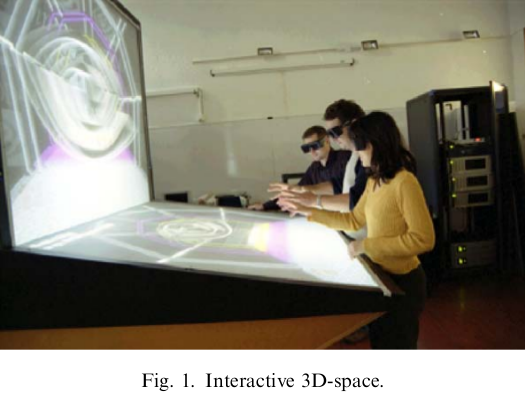
\includegraphics[scale=0.4]{Workspace1.png}
 \begin{itemize}
\item Workbench
\item Two projection screen
\item Camera stereo pair 
\end{itemize}
\framesubtitle{}

\end{frame}

%------------------- Slide ------------------------------
\begin{frame}
\frametitle{Motivation and Context}
 \begin{itemize}
\item Many previous related works have presented a different and various methods of motion tracking most of them required special equipment 
 so it was a challenge for the author to come up with a new method that dose the same job with a almost the same accuracy  but without all the complicated equipment to make it more user friendly    
	
\end{itemize}
\framesubtitle{}

\end{frame}

%------------------- Slide ------------------------------
\begin{frame}
\frametitle{Research Questions}
\framesubtitle{}
\begin{itemize}
\item Is it possible to make a 3D tracking system without the need for the user to put on any special suits or other equipment?? 
\item If yes, then how can we replace these equipment ???  
\end{itemize}
	
\end{frame}

%------------------- Slide ------------------------------
\begin{frame}
\frametitle{Critical Literature Review}
\framesubtitle{}
\begin{itemize}
\item Advantages and Disadvantages.
\item Focusing on different matters at the same time. 
\end{itemize}

\end{frame}

%------------------- Slide ------------------------------
\begin{frame}
\frametitle{Research Method and Results}
\framesubtitle{}
{\huge  What does the system do?} \\
\begin{itemize}
\item  Hands and face tracking algorithm \\
	\begin{enumerate}
	\item Skin-color segmentation module
	\item Date association module
	\item 3D-point reconstruction
	\end{enumerate}

\end{itemize}

\end{frame}

%------------------- Slide ------------------------------

\begin{frame}
\frametitle{Research Method and Results }
\framesubtitle{Skin-color segmentation module}
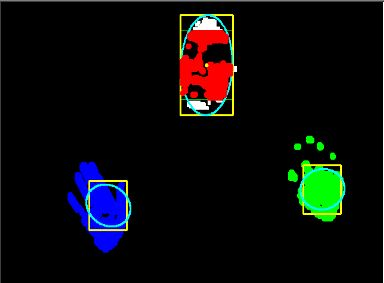
\includegraphics[scale=0.8]{track.jpg}

\end{frame}

%------------------- Slide ------------------------------

\begin{frame}
\frametitle{Research Method and Results }
\framesubtitle{Date association module}
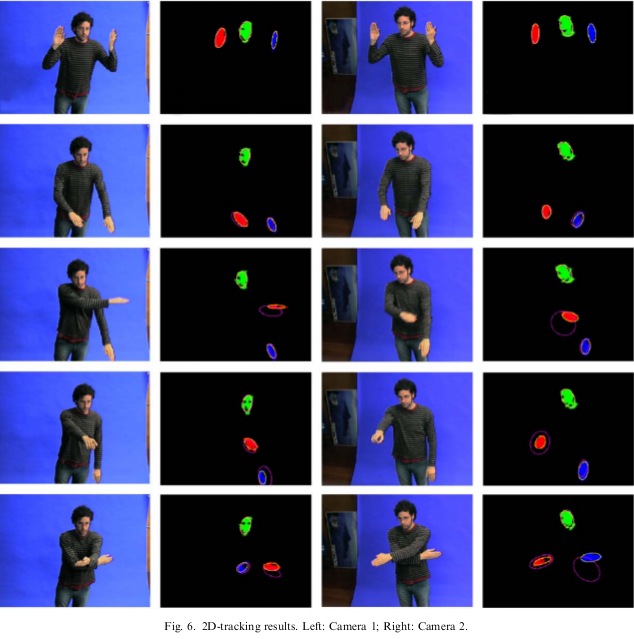
\includegraphics[scale=0.35]{Workspace2.png}

\end{frame}

%------------------- Slide ------------------------------


\begin{frame}
\frametitle{Research Method and Results }
\framesubtitle{3D-point reconstruction}
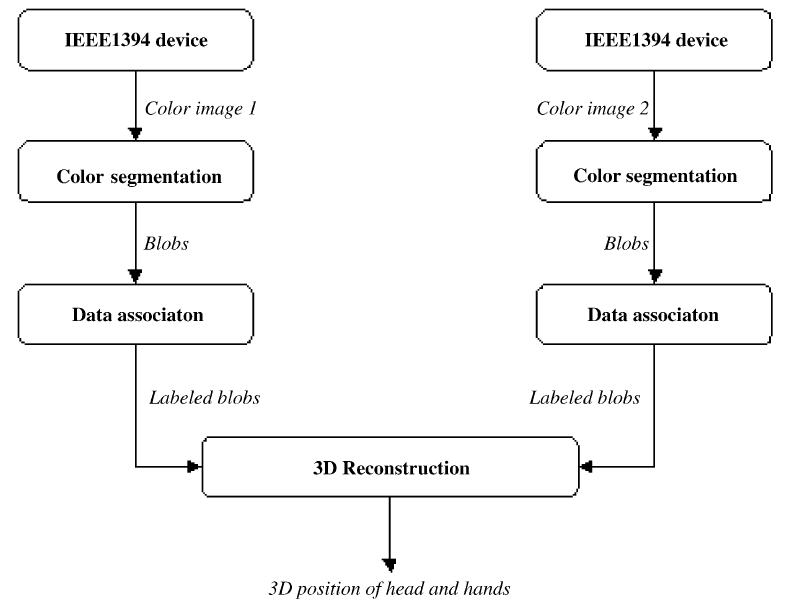
\includegraphics[scale=0.3]{Workspace3.png}

\end{frame}

%------------------- Slide ------------------------------
\begin{frame}
\frametitle{Conclusion }
\framesubtitle{}
We Conclude that: 
\begin{itemize} 
\item The author came up with new method for 3D motion tracking (the special things about it) :
	\begin{itemize}
	\item No special suits or markers are needed (more freedom for the user) 
	\item cost much less than the previous methods
	\end{itemize} 
\item The algorithm for the face and hands tracking is consist of three parts:
 	\begin{itemize}
	\item Skin-color segmentation module
	\item Date association module
	\item 3D-point reconstruction
	\end{itemize} 
\end{itemize}
\end{frame}

%------------------- Slide ------------------------------
\begin{frame}
\frametitle{Q and A}

\Huge Questions And Answers
\framesubtitle{}

\end{frame}

\end{document}